\begin{figure}[!htb]
   \centering
   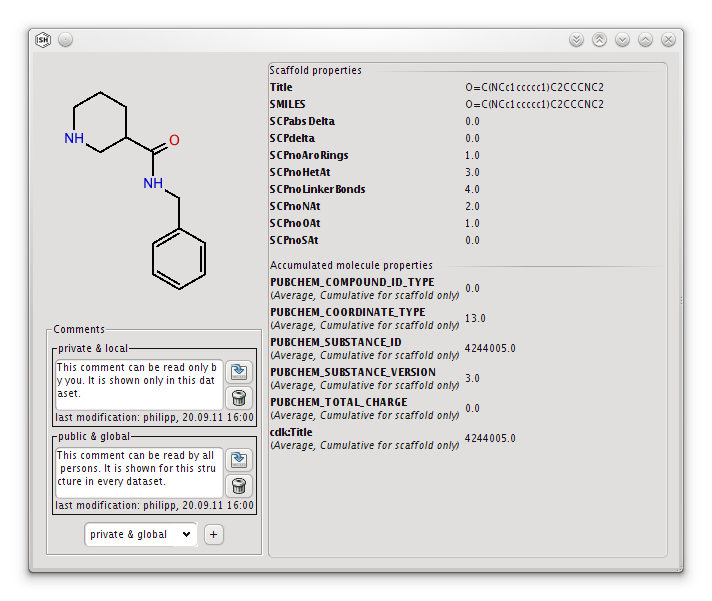
\includegraphics[width=0.5\textwidth]{images/sh_tooltip_dialog.png}
   \caption{Tooltip}
   \label{fig:tooltip}
\end{figure}
An interactive tooltip window (see \figref{fig:tooltip}) is available for the \stview and the \dview when you move your mouse over a molecule or scaffold. It combines the following components in one window. 
\begin{itemize}
 \item a large \textbf{image} of the structure
 \item configurable information on the \textbf{properties}
 \item a component to view, add, delete or modify \textbf{comments}
\end{itemize}
The window behaves different from a normal tooltip in some circumstances. Like a normal tooltip it disappears as soon as the mouse leaves molecule, scaffold or tooltip window. But if you click inside the window the window will stick and stay until the focus of the window is lost. This enables you to move around the mouse freely and (more important) lets you edit the comments more safely.

\subsection{Configuring the Tooltip}
You can find some general options at \texttt{Session $\rightarrow$ Preferences $\rightarrow$ General Configuration} in the menu bar. 
\begin{itemize}
 \item \textbf{enable/disable} tooltip
 \item the \textbf{size} of the image shown in the tooltip
 \item whether it shows \textbf{undefined properties} or not
 \item the \textbf{delay} after which the tooltip is shown
\end{itemize}

\subsection{Configuring the Properties}

\begin{figure}[!htb]
   \centering
   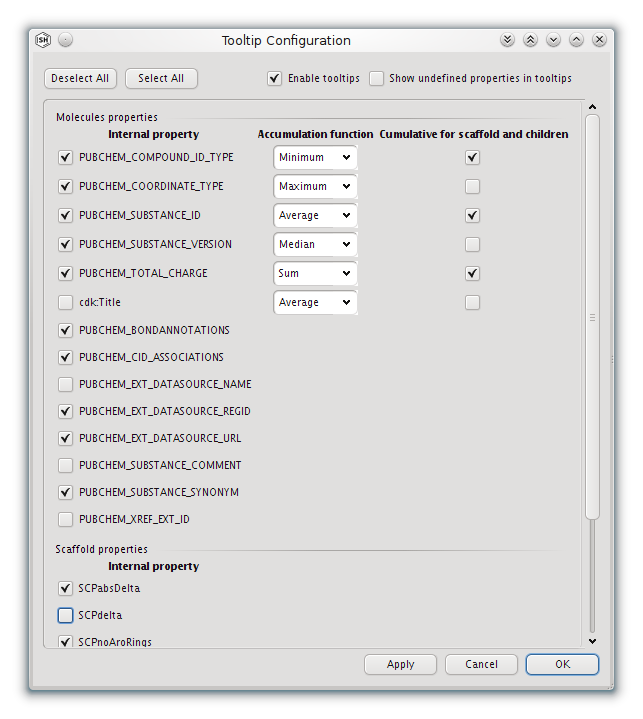
\includegraphics[width=0.5\textwidth]{images/sh_tooltip_configuration_dialog.png}
   \caption{Tooltip Configuration}
   \label{fig:tooltip_configuration}
\end{figure}

You can find a dialog to configure the properties at \texttt{Session $\rightarrow$ Tooltip Configuration} in the menu bar. As you can see in \figref{fig:tooltip_configuration} you have a check box in front of every property to enable or disable the property in the tooltip. As the tooltip can be shown for molecules and scaffolds there are two types of properties. If the tooltip is displayed over a molecule only the molecule properties will be shown. 

The properties for scaffolds are somewhat more complex. You can derive accumulated properties for scaffolds from the molecule properties that belong to the displayed scaffold. Therefore you can choose an accumulation function for each numerical molecule property. For example you can display the average, minimum or maximum of the molecule property when using the tooltip with scaffolds. 
If you enable the checkbox \texttt{Cumulative for scaffold and children} this accumulation function is applied to the molecules of the scaffold and all molecules that belong to any child scaffold.

\subsection{Comments}
You can add, modify and delete comments for a molecule or scaffold directly in the tooltip. You can find the controls in the bottom left corner of the tooltip (see \figref{fig:tooltip}). 

\paragraph{Private, public, local and global comments}
Comments can be private or public and local or global. Therefore you have 4 different types of comments (private \& local, private \& global, public \& local, public \& global). If a comment is private it is only accessible by the user who created it, while a public comment can be seen by any other user working on the same database. If a comment is local it is limited to the current tree. If you choose global instead it will be visible for all datasets and all trees on the current database for molecules or scaffolds with the same structure.

\paragraph{Add, modify or delete a comment}
To add a new comment select the type in the drop-down box and click the plus button. Note that only one comment of each type can exists for each molecule or scaffold. Therefore not all or no types may be available in the drop-down box. After adding a new comment a text field with a save button, delete button and some information about the modification will appear. You can now modify the (empty or previously existent) comments by editing the text in the text field and pressing the save button afterwards. The save button will be only accessible if you already modified the text. Otherwise it will be greyed out. To delete a comment simply press the delete button. The text field with the according controls will disappear.
